\section{Order}
\label{sec:order}

\begin{figure}
	\centering
  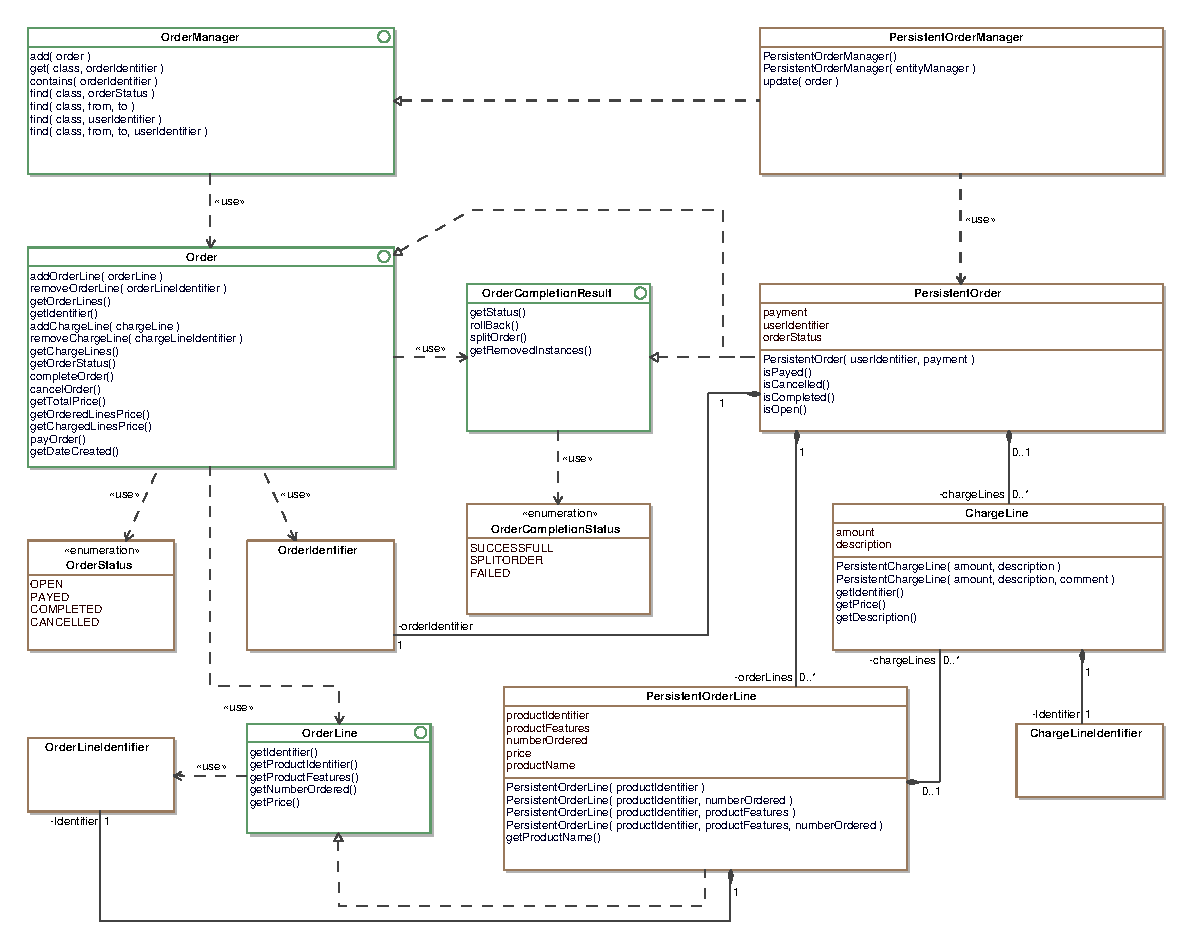
\includegraphics[height=1.0\textwidth,angle=90]{images/Order_Overview.eps}
	\label{order_overview}
	\caption{Order - Class Overview}
\end{figure}
%An Order is a new concept in \salespoint, replacing databaskets from earlier versions.
%An Order provides facilities for individual pricing of products (additional costs or deductions) and state information and manipulation.

An \code{Order} can be considered as a sheet of paper which basically consists of lines, each representing an ordered product.
%(\code{OrderLine}) and lines that are not bound to a concrete product but which cause a charge (\code{ChargeLine}), for example shipping and packaging.
An order can be uniquely identified by an \code{OrderIdentifier}.

Every product of an order is stored in a separate \code{OrderLine}.
An \code{OrderLine} in turn is uniquely identified by an \code{OrderLineIdentifier}.
An \code{OrderLine} contains all information to identify a \code{ProductInstance} (see Section \ref{sec:product}).
A \code{ProductInstance} is identified by a \code{ProductIdentifier}, and an optional set of \code{ProductFeature}s.
\\

A \code{ChargeLine} represents additional costs or discounts and can be applied to an \code{OrderLine} or an \code{Order}. 
For example, \code{ChargeLine}s can be used to handle special taxes or handling fees.
A \code{ChargeLine} is uniquely identified by a \code{ChargeLineIdentifier}.
%ChargeLines will be involved in price calculation of \code{Order}s and \code{OrderLine}s.
\\

\code{Orders} are lifecycle-objects.
The lifecycle covers four states which are defined by enumeration type \code{OrderStatus}.
%The lifecycle has restrictions in changing states, which are transposed automatic by the according methods.
%Changing lifecylce states is restricted, which is automatically governed by the according methods, for example \code{cancelOrder()}.
The lifecycle state cannot be arbitrarily changed, but follows a fixed scheme and is represented as field \code{orderStatus} in the class \code{PersistentOrder}.
State transistions are automatically carried out when certain methods are called on an \code{Order} object, for example \code{cancelOrder()}.
%The figure \ref{order_statemachine} shows a state machine which illustrates the lifecycle of \code{Orders}.
\\


As you can see in Figure \ref{order_statemachine}, a PersistentOrder can only be modified in state \code{OPEN}.
\code{PAYED}, \code{CANCELLED} and \code{COMPLETED} \code{Orders} are immutable.
Calling the \code{payOrder()} method changes the state and calls the accountancy to create a \code{ProductPaymentEntry}
Ordered objects will only be removed from inventory when the \code{completeOrder()} method is called.  
\code{COMPLETED} is one of the final states and it is not possible to change the state of such orders.
\\
\begin{figure}
	\centering
  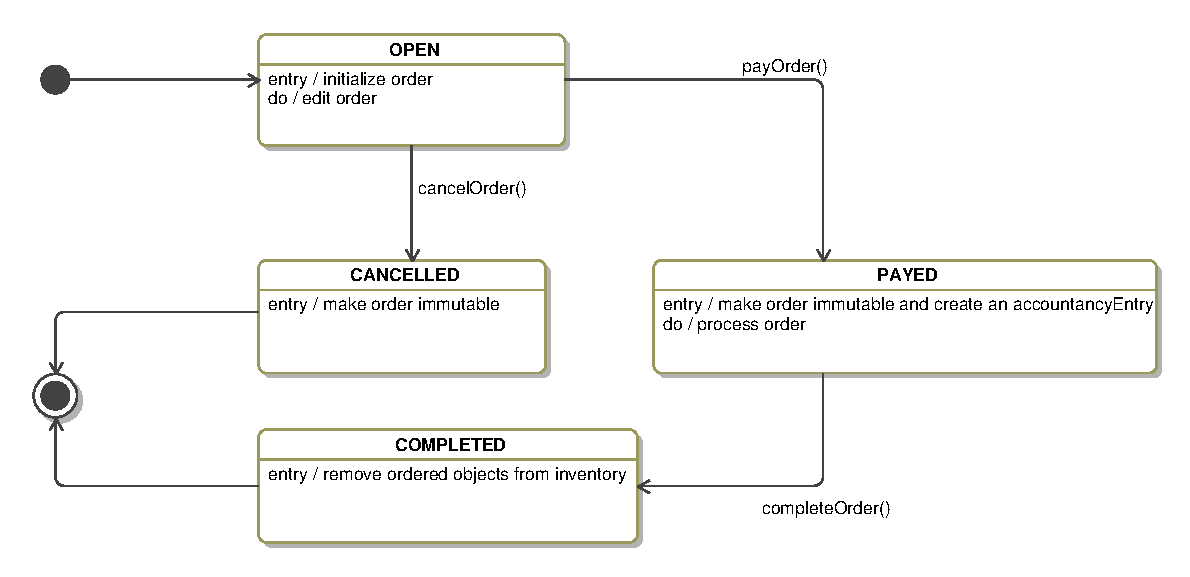
\includegraphics[width=1.0\textwidth]{images/Order_StateMachine.eps}
  \label{order_statemachine}
	\caption{Order - Lifecycle}
\end{figure}  

Completing an order causes product instances to be removed from the inventory.
Because product instances may not be present anymore in the inventory, or their number may not be suffice to fulfill an order, completing an order requires special attention.
To handle these situations, the \code{OrderCompletionResult} interface was introduced.
First of all, three \code{OrderCompletionStatus} are possible:

\begin{itemize}
\item \code{SUCCESSFUL}: The order was completed successfully, and all products were removed from the inventory. 
\item \code{SPLIT}: Some products could be found in the inventory and were removed.
\item \code{FAILED}: An error from which recovery is impossible occured.
\end{itemize}

When completing an order results in the \code{SPLIT} status, the original order is splitted: all product that could be removed from the inventory are kept in the original order.
The original order's state is changed to \code{COMPLETED}.
All products which could not be removed from the inventory are transferred to a second order, the split order. The split order is set to \code{PAYED}.
This scheme allows for the Controller to implement whatever logic necessary: placing a product on back order, splitting the order into multiple deliveries, or cancelling the order.
It is paramount to understand, that \code{OrderCompletionResult} does not make a decision, but prepares for every decision, the business logic may come to.
\\

The \code{OrderManager} aggregates \code{Order}s.
The implementations \code{PersistentOrderManager}, \code{PersistentOrder}, and \code{PersistentOrderLine} are used to persist, update, find and remove orders to/from the database.
In \code{Order} aggregated objects, like \code{OrderLine}s and \code{ChargeLine}s will also be persisted, updated or removed with the \code{Order} object.

